% ! TeX program = xelatex
\documentclass[11.5pt]{beamer}
\usetheme{metropolis}
\usepackage{tabularx}
\usepackage{changepage}
\usepackage{float}
\usepackage{ragged2e}
\usepackage{amsmath}
\usepackage{graphicx}
\usepackage{appendix}
\usepackage[round]{natbib}   % omit 'round' option if you prefer square brackets
\bibliographystyle{aer}

\usepackage{xeCJK}
\setCJKmainfont{regular}[
    Path="../fonts/simplified_chinese/noto_serif/",
    BoldFont=bold.otf
]
\xeCJKDeclareSubCJKBlock{Hangul}{"1100 -> "11FF, "3130 -> "318F, "A960 -> "A97F, "AC00 -> "D7AF, "D7B0 -> "D7FF}
\setCJKmainfont{regular}[
    Hangul,
    Path="../fonts/korean/noto_serif/",
    BoldFont=bold.otf
]

\xeCJKDeclareSubCJKBlock{Kana}{"3040 -> "309F, "30A0 -> "30FF, "31F0 -> "31FF, "1B000 -> "1B0FF}
\setCJKmainfont{regular}[
    Kana,
    Path="../fonts/japanese/noto_serif/",
    BoldFont=bold.otf
]



\title{\huge{Introduction Of Utilizing LLM on Resrearch}}
\author{Hsiu-Hsuan(Jacky) Yeh}
\date{2024-01-26}
\begin{document}
\maketitle


\begin{frame}{Outline}
\tableofcontents
\end{frame}

\section{LLM}
\begin{frame}{List of LLMs}
\begin{itemize}
    \item ChatGPT 3.5/4
    \item Claude 2
    \item Gemini Pro 1.5/Ultra
    \item Llama 2, \cite{Touvron2023}
    \item Mistral 7B, \cite{Jiang2023} 
    \item Falcon 180B, \cite{Almazrouei2023}
\end{itemize}
\end{frame}

\section{In Context Learning}
\subsection{Few-Shot Learning}
\begin{frame}{Few-Shot Learning, \cite{Brown2020}}
LLM can significantly improve task-agnostic few-shot learning performance,
achieving strong results on a variety of NLP tasks without task-specific tuning.
The study contrasts GPT-3's few-shot capabilities with zero-shot and one-shot
settings, showing it can perform competitively with or even exceed
state-of-the-art models that have been fine-tuned for specific tasks.
\end{frame}


\begin{frame}
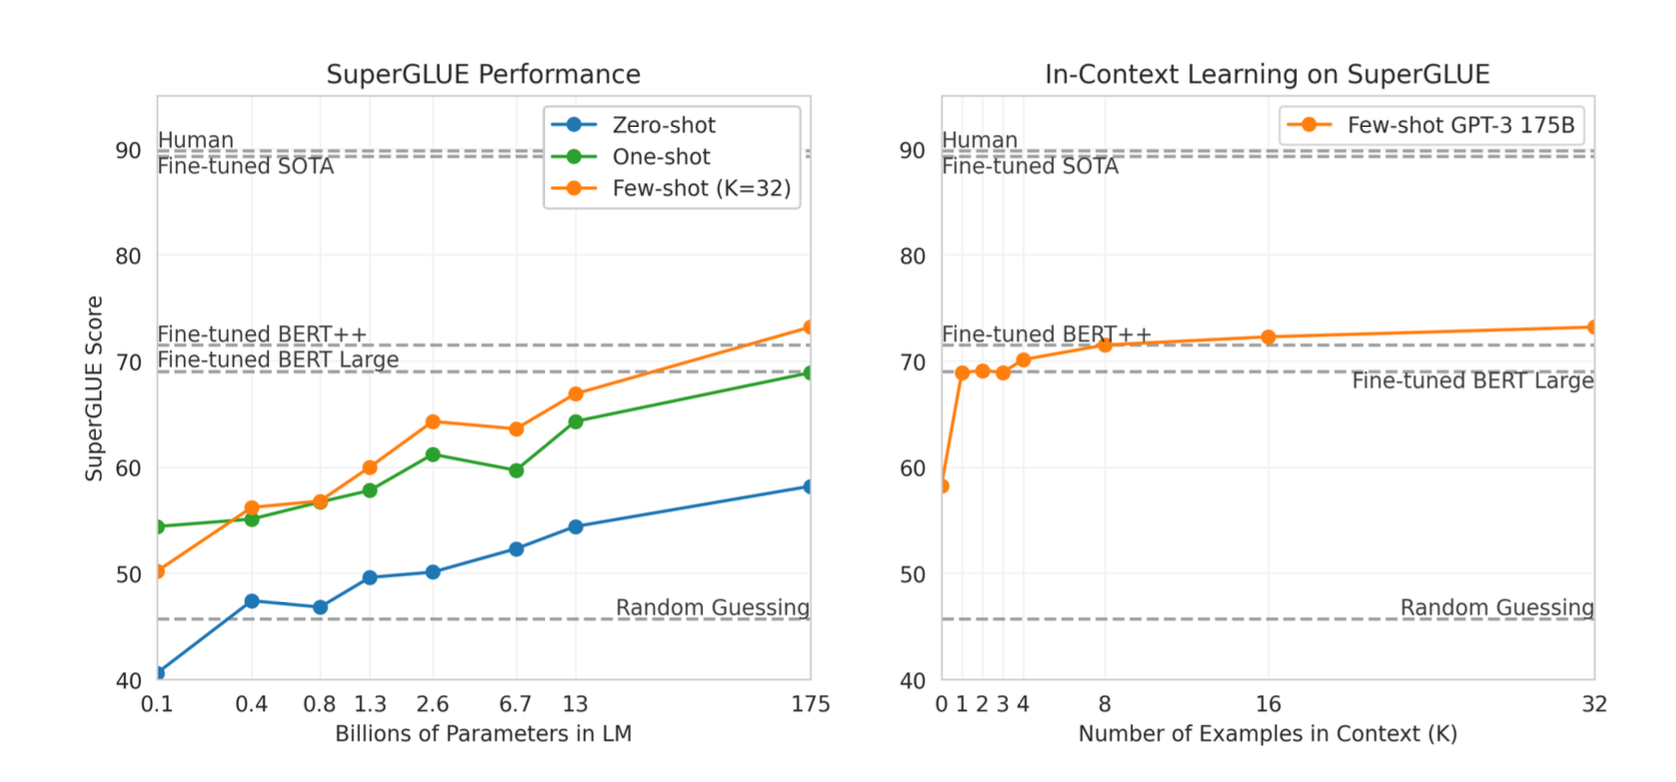
\includegraphics[width=11cm]{Figures/fig1.png}
\end{frame}

\begin{frame}
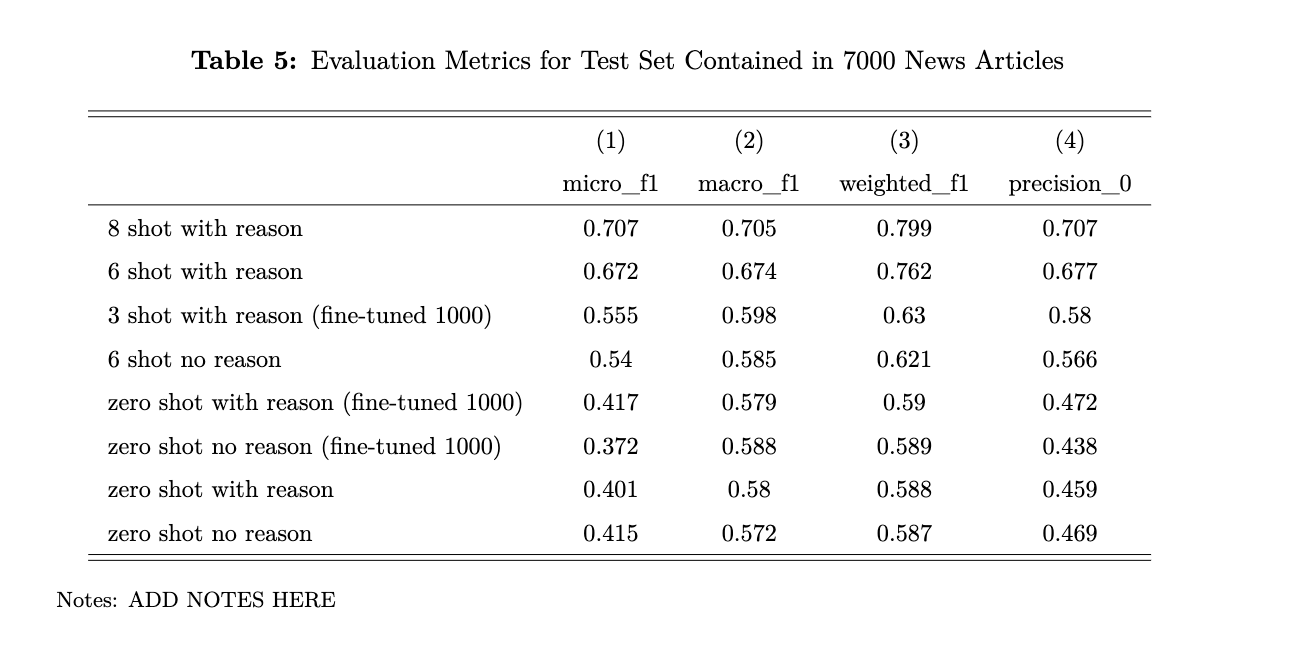
\includegraphics[width=11cm]{Figures/fig2.png}
\end{frame}


\subsection{Chain-of-Thought}
\begin{frame}{Chain-of-Thought, \cite{Wei2022}}
CoT involves providing the model with a few exemplar prompts that
demonstrate the reasoning process step by step, leading to the final answer.
It has been shown to improve performance across a variety of tasks,
including arithmetic, commonsense, and symbolic reasoning, by making the
models' thought process more interpretable and allowing them to tackle
multi-step problems more effectively.
\end{frame}


\begin{frame}
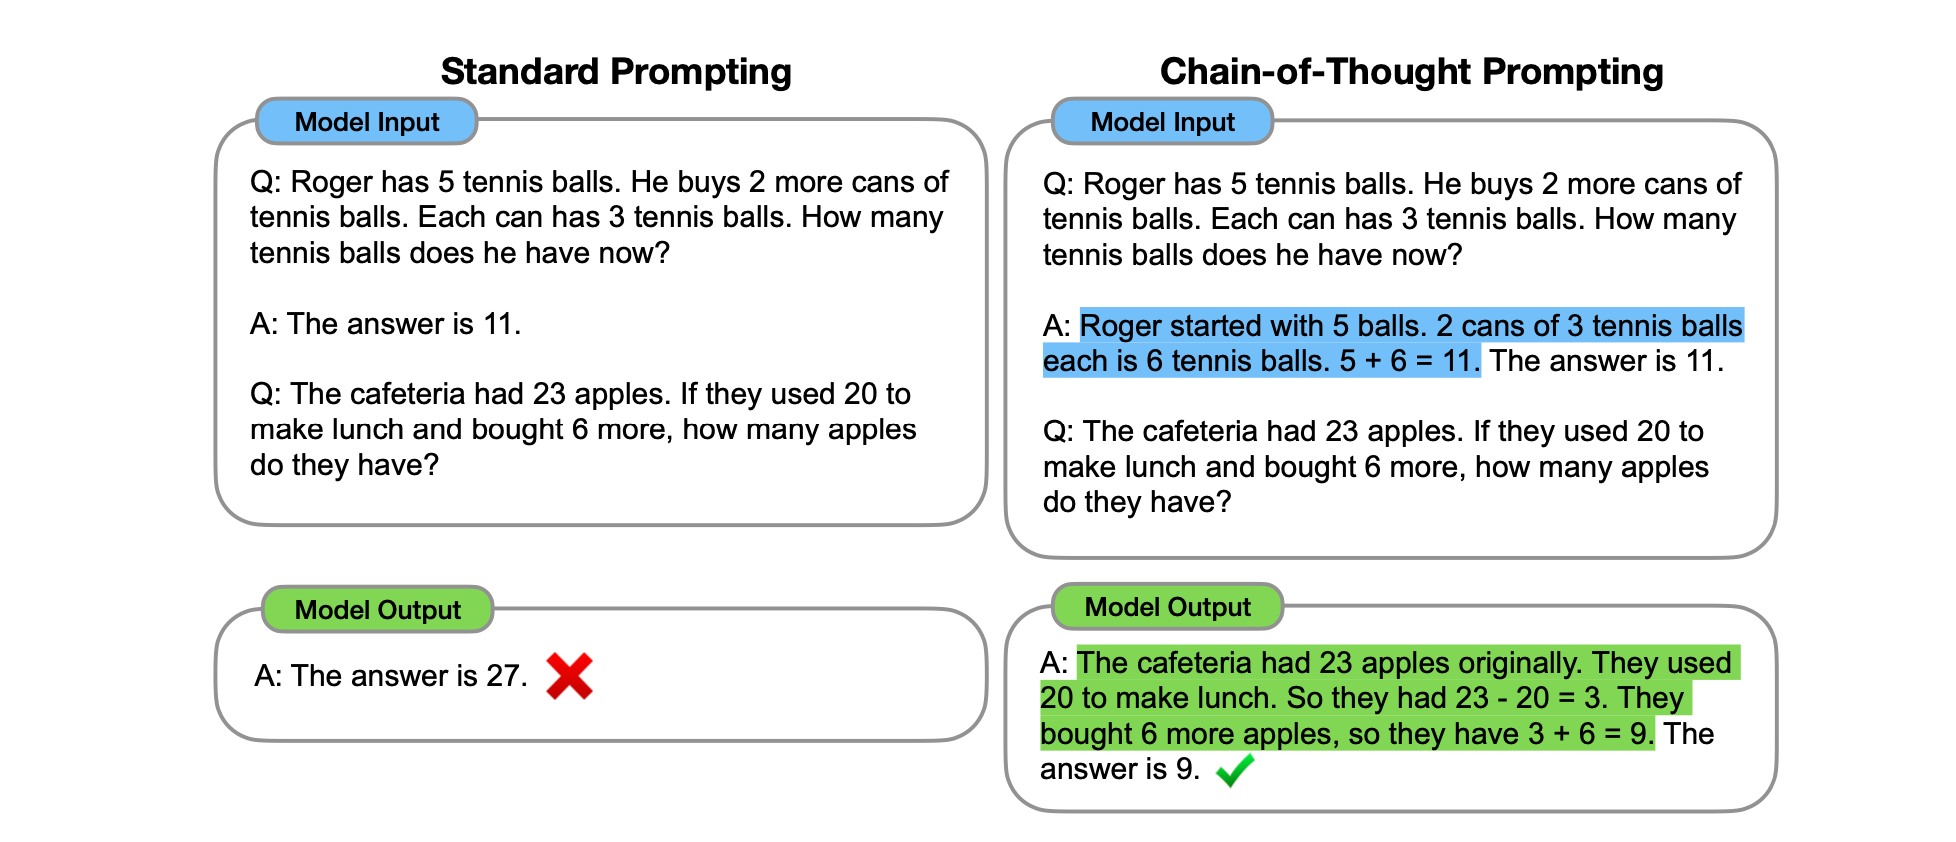
\includegraphics[width=11cm]{Figures/fig3.png}
\end{frame}

\begin{frame}{noise=0}
總統馬英九競選期間提出的募兵支票恐怕面臨跳票?國防部長陳肇敏昨在立法院外交國防委員會中表示,推動募兵制的確有困難,且要推動到全面募兵制,「是國防部嚴峻的考驗」。陳肇敏指出,國防預算佔GDP(Gross Domestic Product,國內生產毛額)百分之三,但以現有國軍員額來看,根本不可能達成全面募兵制,因此國軍要再精進是必然方向。而我國走的是一個海島守勢作戰,各軍種人員配比都要進行檢討,並將繼續推動「再精進案」,將目前二十七萬大軍減至二十到二十五萬人以內。陳肇敏並指出,目前募得許多素質相當不錯的國軍弟兄,主要與過去八年經濟不景氣,工作難找有關,未來經濟好轉後,是否還有誘因?另外,台灣人口有限,國防部會努力推動募兵制,但不能因滿足「量」的需求而減低「質」的要求。至於重大軍購案,陳肇敏強調向美國購買F-16 C/D戰機有其必要,但其他軍購案如潛艦,因目前我方連採購潛艇的型號都沒有,這部分會再研究,會就作戰需求再作評估。記者王<U+70F1>華
\end{frame}

\begin{frame}{CoT reasoning}
Let's think step by step. First, the news is related to Taiwan's economics as
it points out the relation between the quality of voluntary military and the
Taiwan's economics condtion. Second, the news is related to the policy
regarding the voluntary military service. Finally, the news is related to the
uncertainty as it discuss some possibilities and possible progress of the policy.
This news simultaneously mention economics, policy and uncertainty. Hence,
it should not be excluded when constructing Taiwan's EPU index.
\end{frame}


\subsection{Step-Back Prompting}
\begin{frame}{Step-Back Prompting, \cite{Zheng2023}}
This prompting technique improves reasoning in large language models (LLMs)
by leveraging abstraction. This method prompts LLMs to first derive high-level
concepts or principles from detailed questions before addressing the original
query.
\end{frame}

\begin{frame}{Case Study}
User: \newline
Is this article related to economic policy uncertainty? Answer in 30 words. \newline
\{ news \}

LLM(Mistral 7B): \newline
This article discusses Taiwan's defense budget and the challenges of
implementing a full-scale conscription policy, with Defense Minister Chen
Chwen-min stating that it is a severe test for the National Defense Ministry. \newline
... \newline
Regarding major procurement projects, Minister Chen emphasized the necessity
of purchasing F-16 C/D fighter jets from the US, but other procurement cases
like submarines will be studied further based on operational needs.
\end{frame}

\begin{frame}
User: \newline
What is an economic policy uncertainty(EPU) index.

LLM(Mistral 7B): \newline
An Economic Policy Uncertainty (EPU) index measures the level of uncertainty
in the economy due to potential government actions that may impact the economy.
It is calculated based on newspaper articles and other sources, using a
pecific methodology developed by Scott R. Baker, Nicholas Bloom, and
Steven J. Davis. The index is constructed as a composite measure of
uncertainty related to fiscal policy, monetary policy, and regulatory policy.
Higher values of the EPU index indicate greater economic policy uncertainty.
\end{frame}


\begin{frame}
User: \newline
Is this article related to EPU? Answer in 30 words. \newline
\{ news \} \newline

LLM(Mistral 7B): \newline
The Economic Policy Uncertainty (EPU) index is a measure of the level of
policy uncertainty in an economy, calculated using data from newspapers and
other sources to identify the number of articles mentioning economic policy
uncertainty. This article does not directly discuss the EPU index, but rather
Taiwan's defense budget and military conscription issues during the
presidential election period.
\end{frame}


\subsection{ReAct}
\begin{frame}{ReAct, \cite{Yao2023a}}
ReAct prompts LLMs to interleave reasoning (generating verbal reasoning traces)
with action (making task-specific actions), thus enabling dynamic adjustment
of plans based on both internal reasoning and external information.
\end{frame}


\begin{frame}
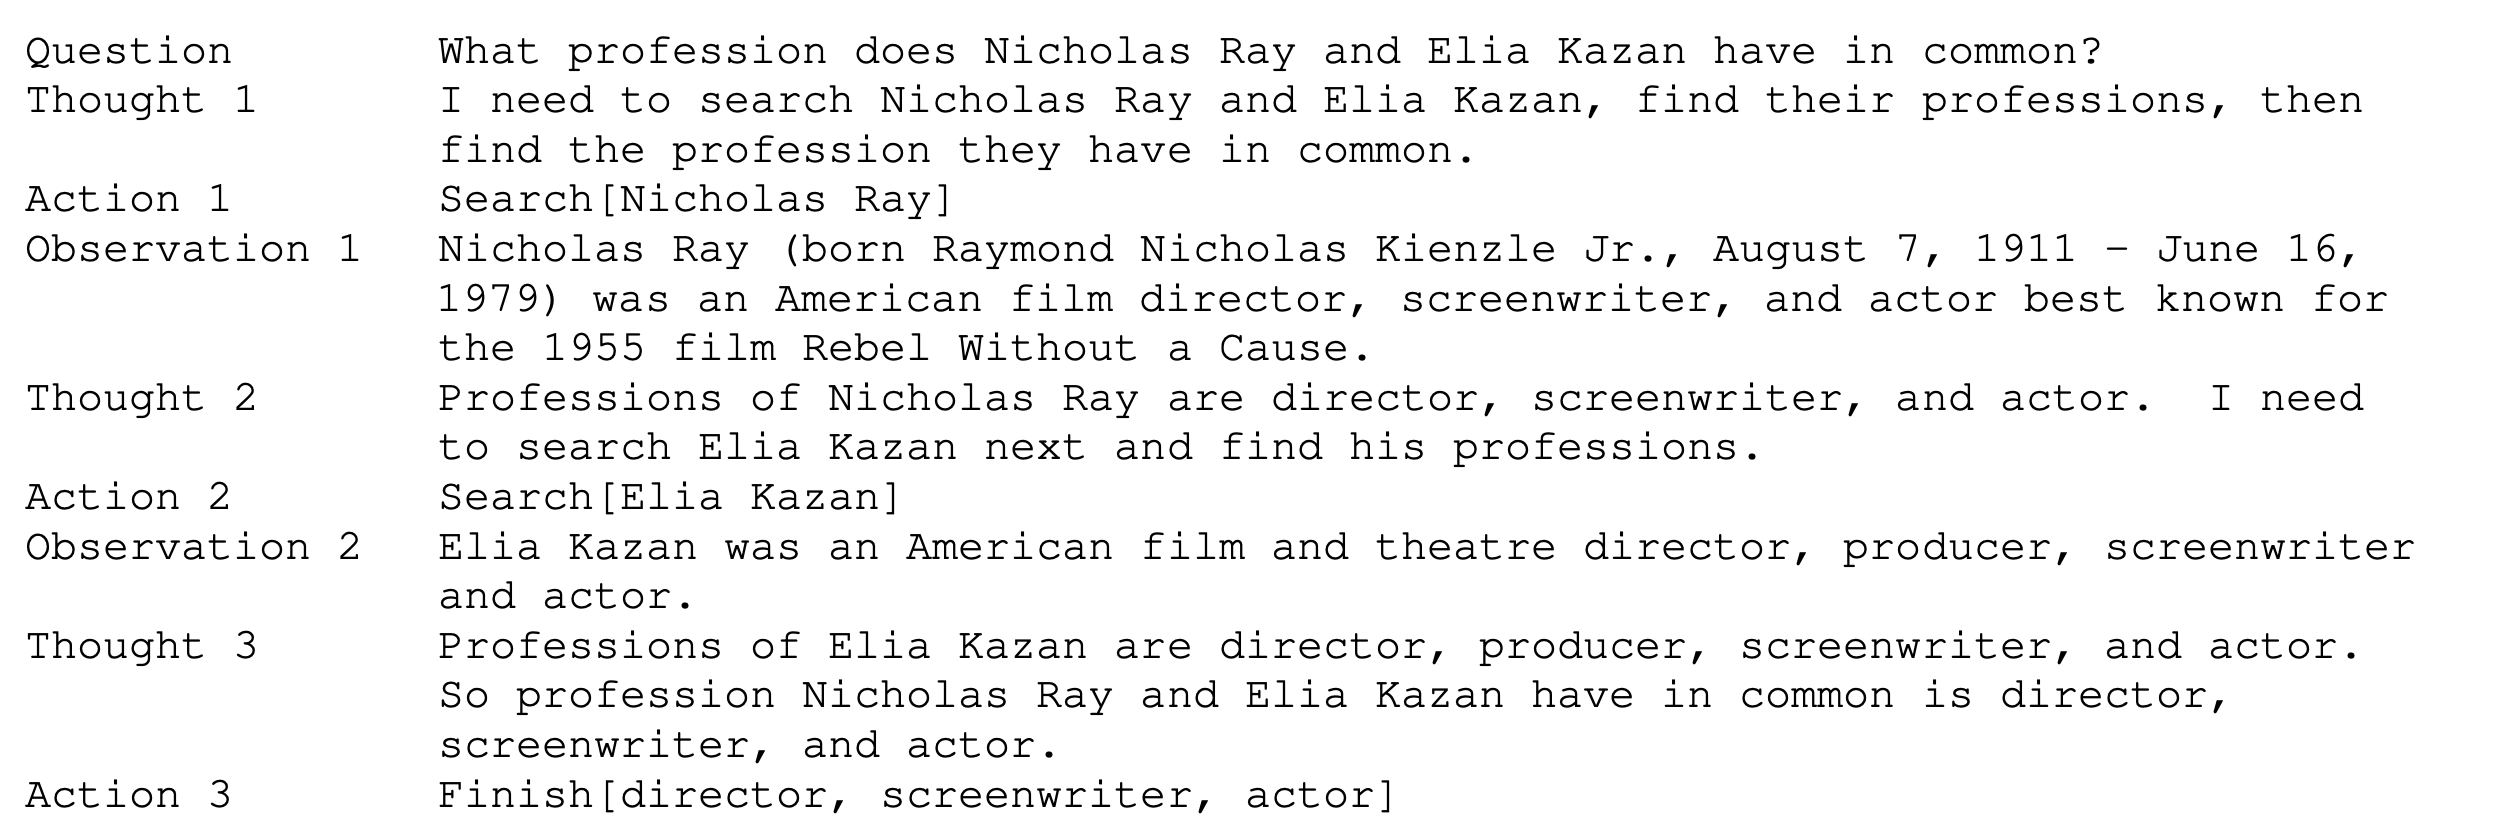
\includegraphics[width=11cm]{Figures/fig4.png}
\end{frame}


\subsection{Medprompt+}
\begin{frame}{Medprompt+, \cite{Nori2023}}
This prompting technique combines dynamic few-shot example selection,
self-generated chain-of-thought reasoning, and choice shuffle ensembling.
MedPrompt showcases the potential of generalist models to achieve
specialist-level performance through carefully engineered prompts,
demonstrating a versatile approach applicable across various domains beyond 
medicine.
\end{frame}


\begin{frame}
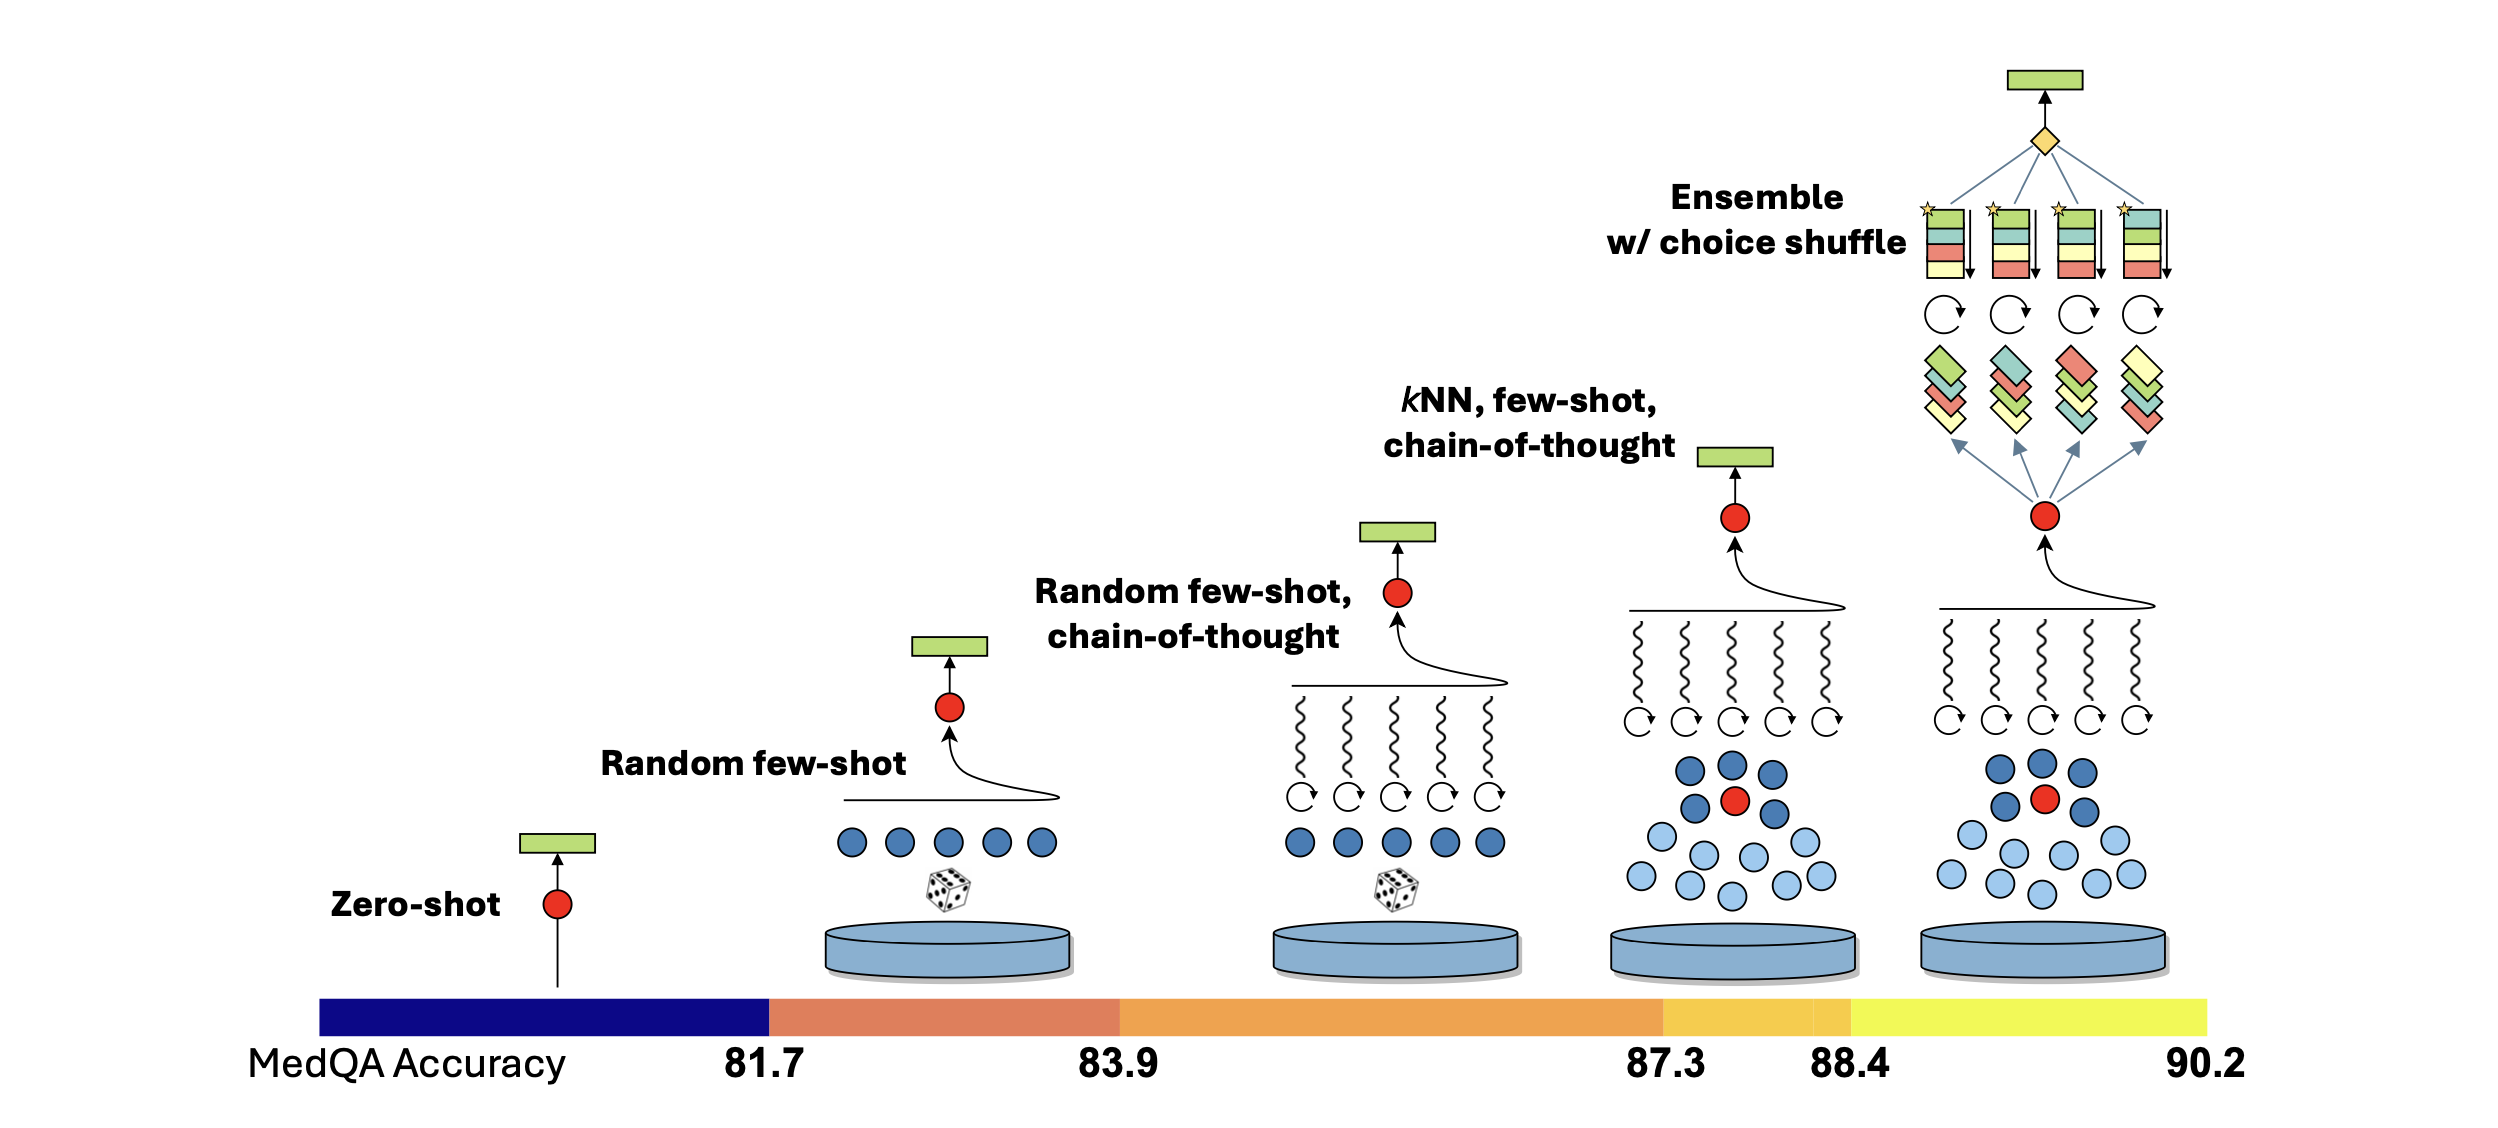
\includegraphics[width=11cm]{Figures/fig5.png}
\end{frame}


\subsection{others}
\begin{frame}{others}
\begin{itemize}
    \item Principles Of Prompting, \cite{Bsharat2024}
    \item Self-Consistency, \cite{Wang2022}
    \item Tree Of Thoughts, \cite{Yao2023}
    \item Self-Discover, \cite{Zhou2024}
\end{itemize}
\end{frame}



\section{Fine-tuning}
\begin{frame}{Wikipedia}
In deep learning, fine-tuning is an approach to transfer learning in which the
weights of a pre-trained model are trained on new data.
\end{frame}
\begin{frame}{Benefit}
Fine-tuning improves on few-shot learning by training on many more examples
than can fit in the prompt, letting you achieve better results on a wide number
of tasks.
Once a model has been fine-tuned, you won't need to provide as many examples
in the prompt.
\end{frame}

\begin{frame}{Documentation}
\href{https://platform.openai.com/docs/guides/fine-tuning}{Documentation}

\href{https://platform.openai.com/docs/api-reference/fine-tuning}{API reference}
\end{frame}


\section{LangChain}
\begin{frame}{LangChain-Core}
The main component of LangChain-Core is LCEL, LangChain Expression Languages,
which involves several sub-components: prompt template, model, output parser,
etc.
\end{frame}


\begin{frame}{Ecosystem}
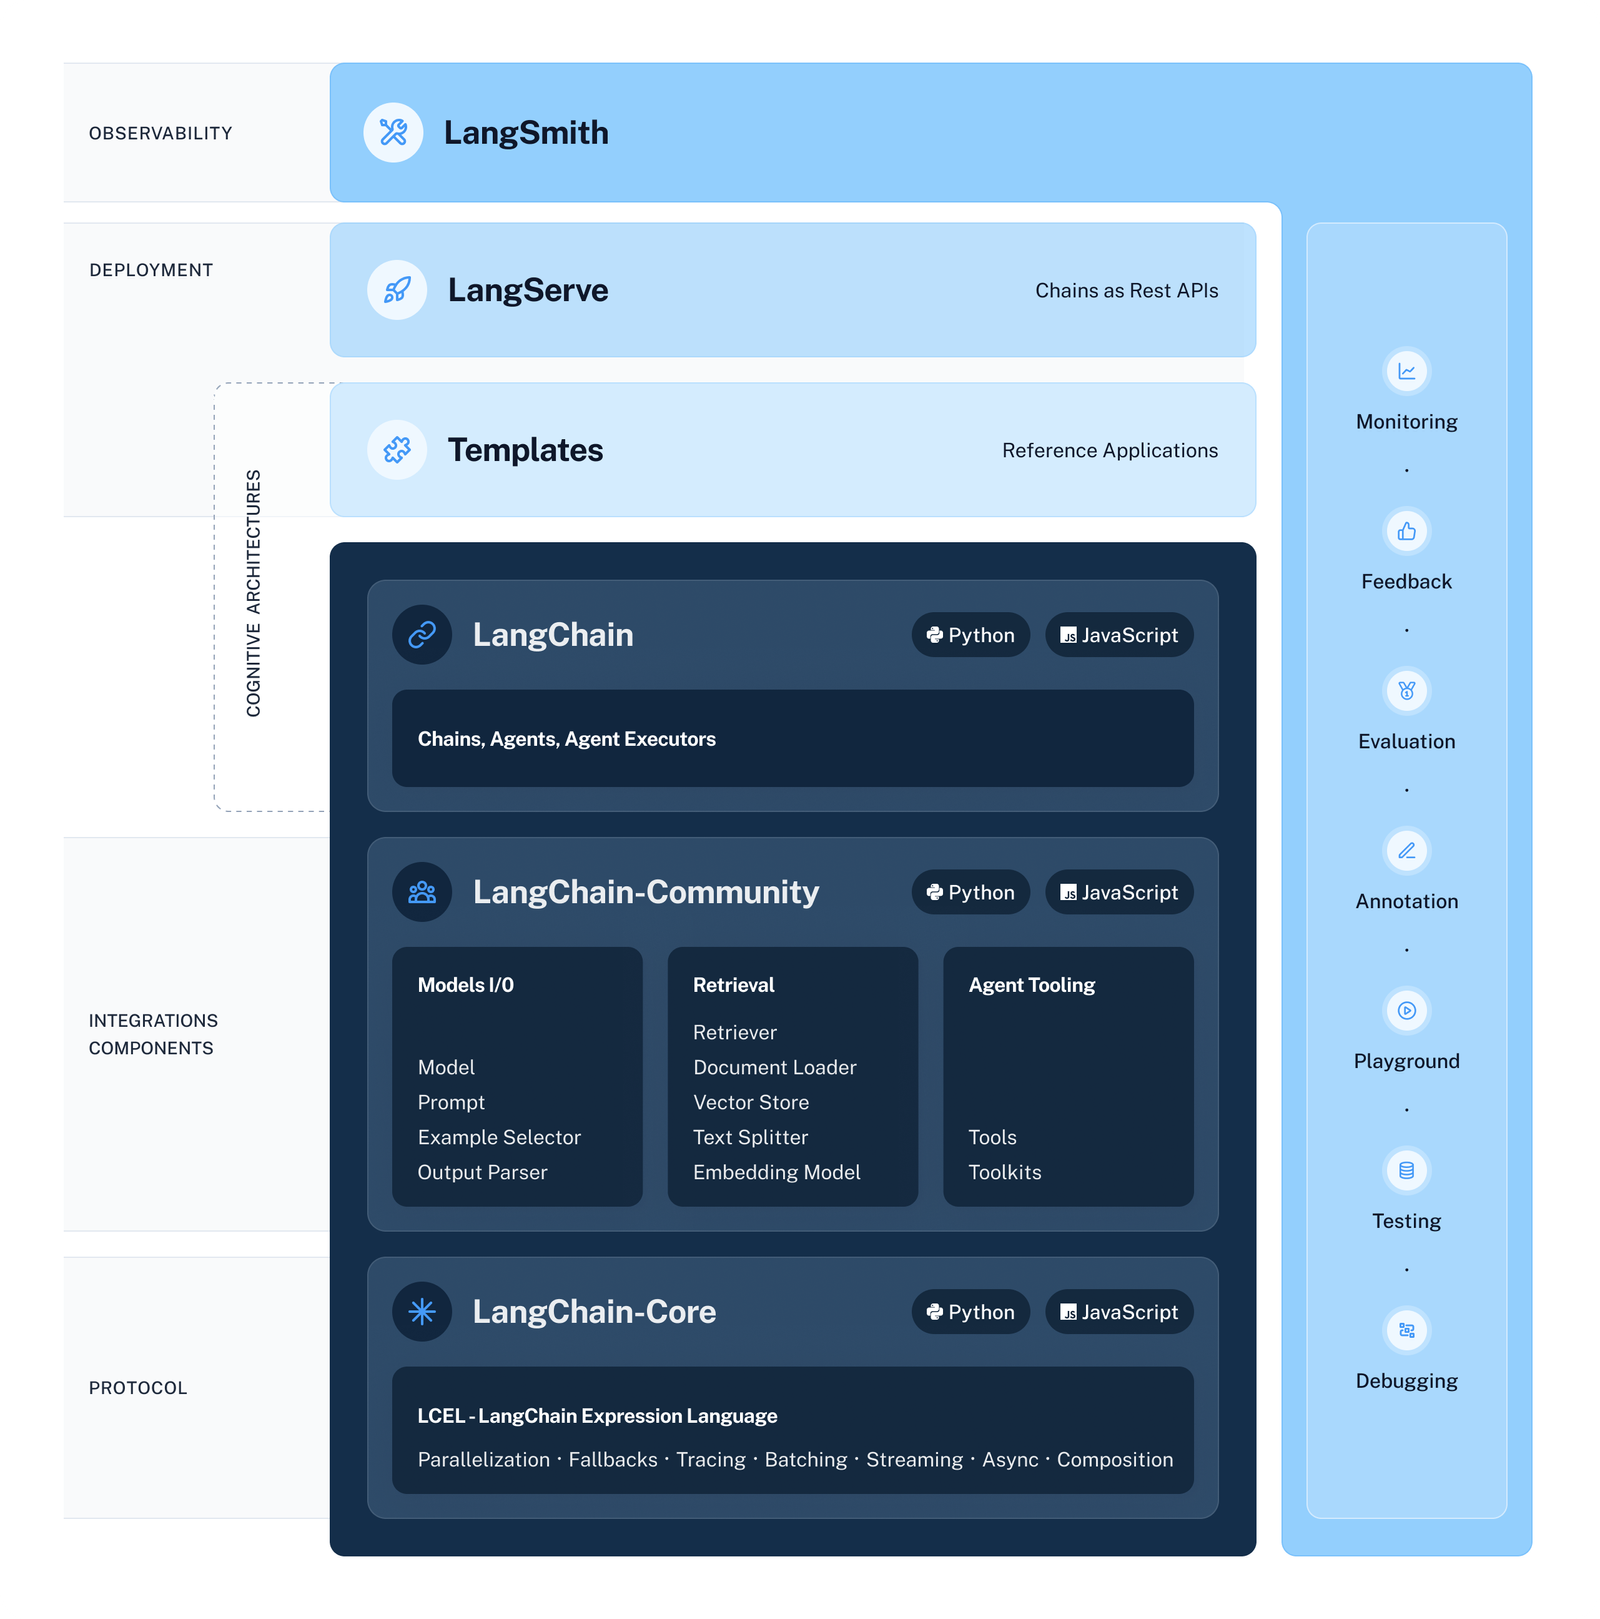
\includegraphics[width=11cm]{Figures/fig6.png}
\end{frame}


\begin{frame}{Prompt Template}
\href{https://github.com/githubjacky/llm-research/blob/main/examples/english_address_to_chinese/main.ipynb}{prompt template example}
\end{frame}


\begin{frame}{LCEL}
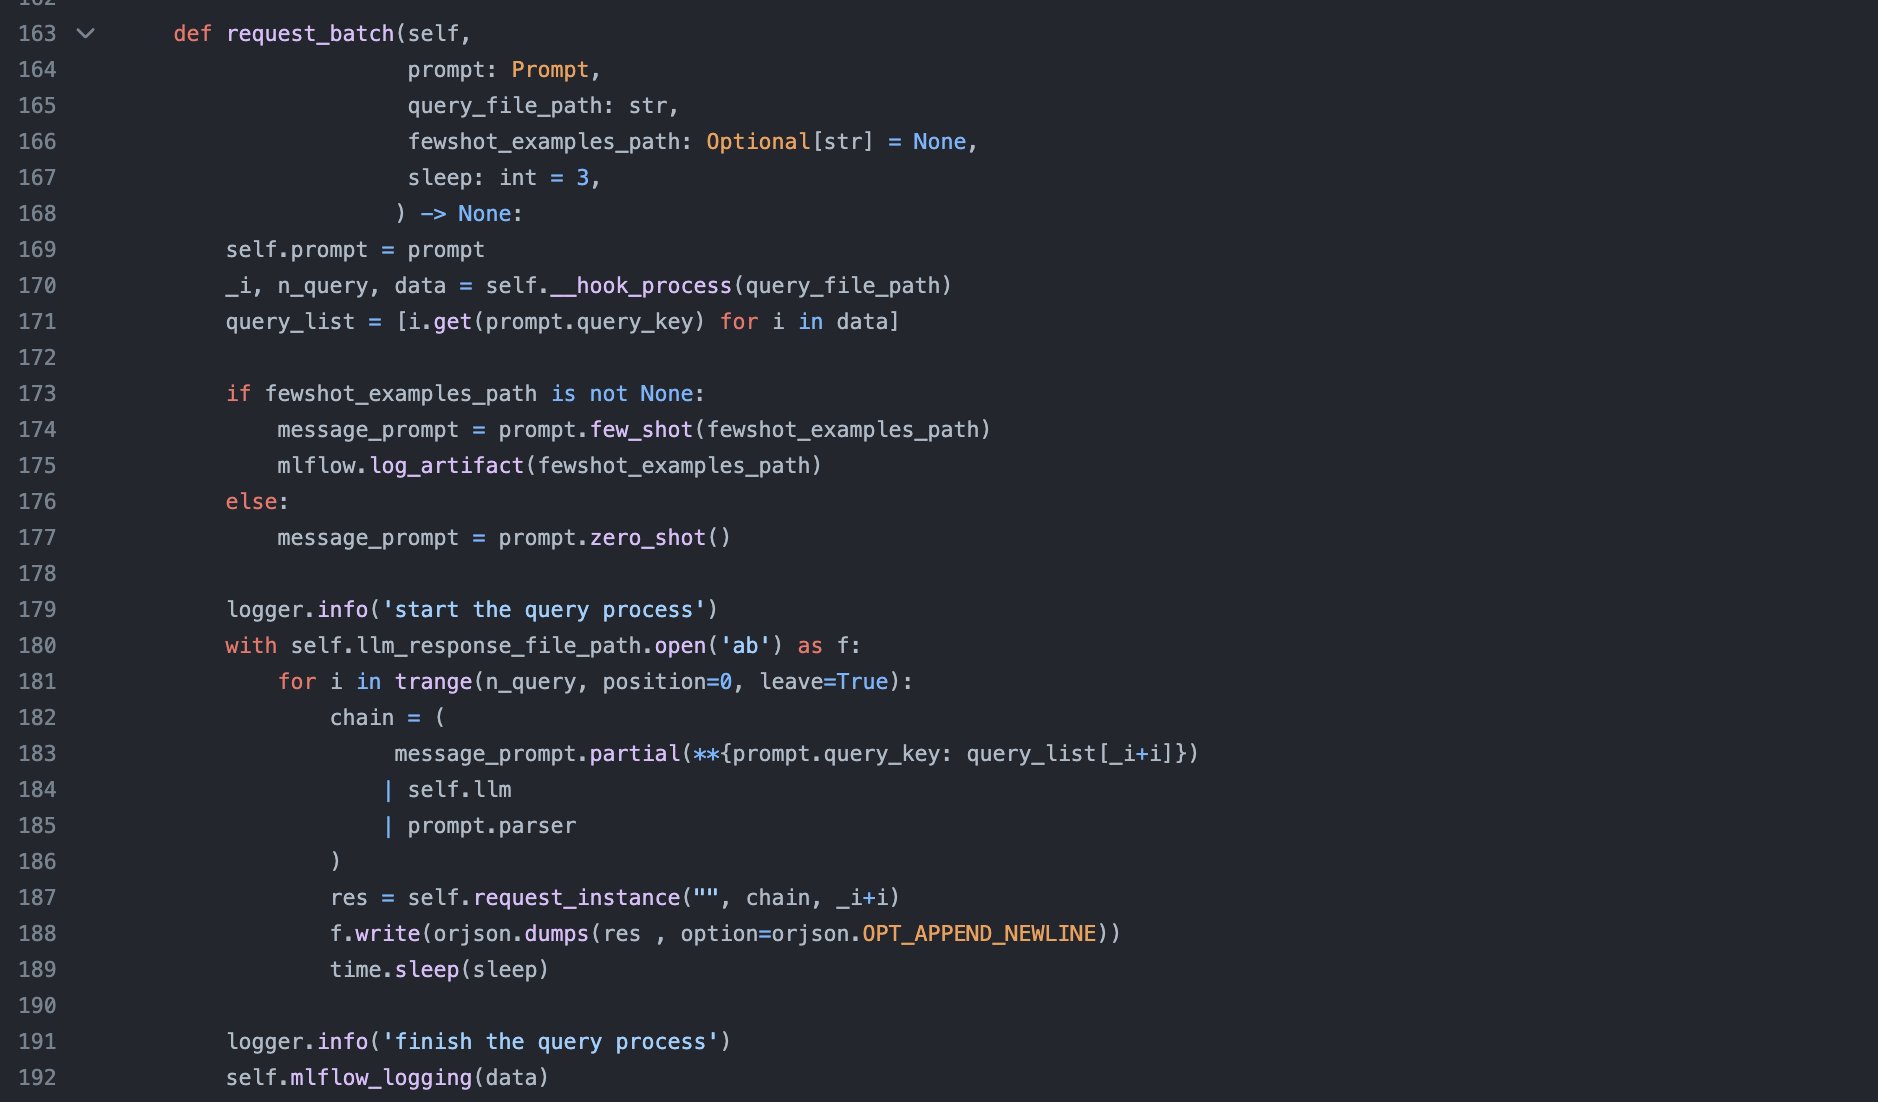
\includegraphics[width=11cm]{Figures/fig7.png}
\end{frame}


\section{References}


\begin{frame}[allowframebreaks]{}
\renewcommand{\section}[2]{}%
\bibliography{/Users/jackyyeh/Library/texmf/bibtex/bib/Zotero.bib}
\end{frame}
\end{document}
